\section{Aufgabe 2} \label{ex2}
In der Aufgabe 2 wurde eine Funktion zum zeichnen eines Quadrates variabler Position und Größe (size) geschrieben. Diese kann 
dann direkt verwendet werden um komplexere Muster mit übergeordnetem Koordinatensystem zu zeichnen, wie z.B. Arcade Figuren.

\subsection{VHDL-Code AXI Schnittstelle}
Wrapper mit Schnittstelle  \\
s\_axi\_interface mit Namenskonvention: <peripheral>\_<version>.vhd
\begin{verbatim}
library ieee;
use ieee.std_logic_1164.all;
use ieee.numeric_std.all;

entity lab3_a1_vga_v2_v1_0 is
	generic (
		-- Users to add parameters here

		-- User parameters ends
		-- Do not modify the parameters beyond this line

		-- Parameters of Axi Slave Bus Interface S00_AXI
		C_S00_AXI_DATA_WIDTH	: integer	:= 32;
		C_S00_AXI_ADDR_WIDTH	: integer	:= 4
	);
	port (
		-- Users to add ports here
        s00_vga_clk  : in std_logic;
        s00_reset    : in std_logic;
        s00_vSync    : out std_logic;
        s00_hSync    : out std_logic;
        s00_red      : out std_logic_vector( 3 downto 0 );
        s00_green    : out std_logic_vector( 3 downto 0 );
        s00_blue     : out std_logic_vector( 3 downto 0 );
		-- User ports ends
		-- Do not modify the ports beyond this line

		-- Ports of Axi Slave Bus Interface S00_AXI
		s00_axi_aclk	: in std_logic;
		s00_axi_aresetn	: in std_logic;
		s00_axi_awaddr	: in std_logic_vector(C_S00_AXI_ADDR_WIDTH-1 downto 0);
		... weitere AXI Signale...
\end{verbatim}

s\_axi Komponente mit VGA Interface  \\
s\_axi\_interface mit Namenskonvention: <peripheral>\_<version>\_<AXI\_instance>.vhd

\begin{verbatim}
library ieee;
use ieee.std_logic_1164.all;
use ieee.numeric_std.all;

entity lab3_a1_vga_v2_v1_0_S00_AXI is
	generic (
		-- Users to add parameters here

		-- User parameters ends
		-- Do not modify the parameters beyond this line

		-- Width of S_AXI data bus
		C_S_AXI_DATA_WIDTH	: integer	:= 32;
		-- Width of S_AXI address bus
		C_S_AXI_ADDR_WIDTH	: integer	:= 4
	);
	port (
		-- Users to add ports here
        vga_clk  : in std_logic;
        reset    : in std_logic;
        vSync    : out std_logic;
        hSync    : out std_logic;
        red      : out std_logic_vector( 3 downto 0 );
        green    : out std_logic_vector( 3 downto 0 );
        blue     : out std_logic_vector( 3 downto 0 );
		-- User ports ends
		-- Do not modify the ports beyond this line

		-- Global Clock Signal
		S_AXI_ACLK	: in std_logic;
		-- Global Reset Signal. This Signal is Active LOW
		S_AXI_ARESETN	: in std_logic;
		-- Write address (issued by master, acceped by Slave)
		S_AXI_AWADDR	: in std_logic_vector(C_S_AXI_ADDR_WIDTH-1 downto 0);
		... weitere Befehle...
...
---------------------------------------------------------------------------------------
---------------------- VGA-Controller RAM und Signale Anfang  --------------------------
    -- RAM
    constant low_address: natural := 0;
    constant high_address: natural := ((640 * 480) - 1); -- 640 * 480 =  307200 --> 
      --Starten bei 0 --> 307199
TYPE ram_type is array (high_address downto low_address) of std_logic_vector (1 downto 0);
    SIGNAL RAM: ram_type;

  signal RAM_address : integer RANGE low_address TO high_address := low_address;
     -- The current Ram Adress
  signal ram_Data    : std_logic_vector(1 downto 0) := "00"; -- The current Ram Data  

    SIGNAL vsynct, hsynct           : std_logic := '1'; -- intermediate sync-signals
    SIGNAL pixel_x_sig, pixel_y_sig : std_logic_vector( 9 downto 0 );
    SIGNAL pixel_x_int, pixel_y_int : integer RANGE 0 TO 1023;
    SIGNAL video_on                 : std_logic;
    
    -- CONSTANT h_active_video         : INTEGER := 640; -- horizontal active video
    -- CONSTANT h_front_porch          : INTEGER := 16; -- horizontal front porch
    -- CONSTANT h_retrace              : INTEGER := 96; -- horizontal retrace / 
         -- sync pulse length
    -- CONSTANT h_back_porch           : INTEGER := 48; -- horizontal back porch
    -- 
    -- CONSTANT v_active_video         : INTEGER := 480; -- vertical active video
    -- CONSTANT v_front_porch          : INTEGER := 10; -- vertical front porch
    -- CONSTANT v_retrace              : INTEGER := 2; -- vertical retrace /
    -- sync pulse length
    -- CONSTANT v_back_porch           : INTEGER := 33; -- vertical back porch

    component vga_sync
    port ( vga_clk  : in std_logic;
           reset    : in std_logic;
           pixel_x  : out std_logic_vector( 9 downto 0 );
           pixel_y  : out std_logic_vector( 9 downto 0 );
           video_on : out std_logic;
           hSync    : out std_logic;
           vSync    : out std_logic);
    end component;  
---------------------- VGA-Controller RAM und Signale Ende -----

...

	-- Add user logic here
    -----------------------------------------------------------------------------
    -----------------------------------------------------------------------------    
    -- Write RAM-Data from AXI-Stream
    -- Get  from AXI-Stream slv_reg0, with the information:
    -- X Position
    -- Y Position
    -- Colour
    -- and write it into the RAM.
    process(S_AXI_ACLK)
        variable x_position   : integer;
        variable y_position   : integer;
        variable RAM_position : integer;
        
       begin
         if rising_edge(S_AXI_ACLK) then    
            x_position := to_integer(ieee.NUMERIC_STD.unsigned( slv_reg0(20 downto 11) ) );
            y_position := to_integer(ieee.NUMERIC_STD.unsigned( slv_reg0(10 downto 2 ) ) );
                          
             RAM_position :=  (x_position + (y_position * 640 ));
                           
             RAM(RAM_position) <= slv_reg0(1 downto 0);                             
        end if;
    end process;    
    ----------------------------------------------------------------------------- 
    
    vga_sync_comp: vga_sync port map (
        vga_clk   => vga_clk,
        reset     => reset,
        pixel_x   => pixel_x_sig,
        pixel_y   => pixel_y_sig,
        video_on  => video_on,
        hSync     => hsynct,
        vSync     => vsynct);
    
    pixel_x_int <= to_integer( unsigned( pixel_x_sig ) );
    pixel_y_int <= to_integer( unsigned( pixel_y_sig ) );
    
    -----------------------------------------------------------------------------
     -- calculate the current RAM address.
     process(pixel_x_int, pixel_y_int)
        begin
        if (video_on = '1') then
            -- calculate the current RAM address.
            RAM_address <= (pixel_x_int + (pixel_y_int * 640));
            --RAM_address <= ( pixel_x + pixel_y );
        end if;
    end process;
    -----------------------------------------------------------------------------
    
    -----------------------------------------------------------------------------
    -- Set the vga_colour_out from the RAM
    process(vga_clk)
        -- variable RAM_position : integer;
        begin
        -- erst bei der fallenden Flanke wird vga_colour_out benoetigt, 
        -- deswegen koennen wir das hier machen.
        if rising_edge(vga_clk) then
            -- Get the RAM Adress from the STD Logic Vector
            ram_Data <= RAM(RAM_address);
        end if;
    end process;
    -----------------------------------------------------------------------------
    
    -----------------------------------------------------------------------------
    process(vga_clk)
        variable  vga_colour_out : std_logic_vector(11 downto 0);
        
        begin
        if falling_edge(vga_clk) then
            if (video_on='1') then
                case ram_Data is     
                    when "00" =>    vga_colour_out := "111100000000" ; 
                        -- vga_colour_out := "111111111111" ; -- Weiss initial
                    when "01" =>    vga_colour_out := "111100000000" ; -- ROT 
                    when "10" =>    vga_colour_out := "000011110000" ; -- GRUEN
                    when "11" =>    vga_colour_out := "000000001111" ; -- BLAU
                    when others =>  vga_colour_out := (OTHERS => '0'); -- TO 0 !!!!!
                end case;
             
                red    <=  vga_colour_out(11 downto 8);
                green   <= vga_colour_out(7 downto 4);
                blue    <= vga_colour_out(3 downto 0);
            else
                red   <= (others => '0');
                green <= (others => '0');
                blue  <= (others => '0');
            end if;
            hSync <= hsynct;
            vSync <= vsynct;
        end if;
    end process; 
    -----------------------------------------------------------------------------
    -----------------------------------------------------------------------------
	-- User logic ends

end arch_imp;
\end{verbatim}

\subsection{C-Code}
C-Code zur Generierung von geometrischen Figuren. Es wurden Quadrate und darauf aufbauend eine Space-Invaders 
Figure kreiert. Zusätzlich können über die Hardware-Switches drei verschiedene Modi umgeschaltet werden:\\
BTN0: Toggle Augenfarbe zwischen rot und blau\\
BTN1: Hintergrundfarbe umschalten zwsichen blau/weiss\\

\begin{verbatim}
/* ------------------------------------------------
 * | UART TYPE   BAUD RATE                      |
 * ------------------------------------------------
 *   uartns550   9600
 *   uartlite    Configurable only in HW design
 *   ps7_uart    115200 (configured by bootrom/bsp)
 */
#include  <stdio.h>
#include  <stdlib.h>
#include  <time.h>

#include "platform.h"
//  Include  Files
#include "xparameters.h"
#include "xgpio.h"
#include "xstatus.h"
#include "xil_printf.h"
#include "lab3_a1_vga_v2.h"

//  Definitions
#define BASE_ADDR 0x43C00000
#define  SW_DEVICE_ID  XPAR_AXI_GPIO_0_DEVICE_ID

#define  LED_DELAY  10000000
#define  LED_CHANNEL 1
#define  printf  xil_printf

XGpio  SWInst; // LEDInst
static int sw_value ;

#define BTN0 1
#define BTN1 2
#define BTN2 4
#define BTN3 8
#define BTN4 16
#define BTN5 32
#define BTN6 64
#define BTN7 128

#define EYE 2
#define BODY 46

typedef enum _color {
	eW = 0,
	eR  = 1,
	eG  = 2,
	eB  = 3
} ecolor;

typedef struct _coord {
	int x;
	int y;
} coord;

// Arcade Figur
uint eyex[EYE] = {3,7};
uint eyey[EYE] = {3,3};
uint spx[BODY] = {2,8,3,7, 2,3,4,5,6,7,8, 1,2,4,5,6,8,9, 
                     0,1,2,3,4,5,6,7,8,9,10, 0,2,3,4,5,6,7,8,10, 0,2,8,10, 3,4,6,7};
uint spy[BODY] = {0,0,1,1, 2,2,2,2,2,2,2, 3,3,3,3,3,3,3, 
                    4,4,4,4,4,4,4,4,4,4, 4, 5,5,5,5,5,5,5,5, 5, 6,6,6, 6, 7,7,7,7};

void paintsquare(uint x, uint y, uint size, ecolor color) {
	if (x < 0 || x > 630)
		return;
	if (y < 0 || y > 470)
		return;
		
	uint i,j;
	for (i = x; i < x+size; ++i)
		for (j = y; j < y+size; ++j)
			LAB3_A1_VGA_V2_mWriteReg((u32)BASE_ADDR, 0, (i << 11 | j << 2 | color));
} 

void resetbg (ecolor color) {
	int i,j;
	for (i = 0; i < 680; ++i)
		for (j = 0; j < 480; ++j)
			LAB3_A1_VGA_V2_mWriteReg((u32)BASE_ADDR, 0, (i << 11 | j << 2 | color));
}

int  main()
{
	double DELAY = 10000000,z;
	init_platform ();
	int status ;

	// Initialise Push Buttons
	status = XGpio_Initialize (&SWInst , SW_DEVICE_ID );
	if ( status != XST_SUCCESS )
		return XST_FAILURE ;
	XGpio_SetDataDirection (&SWInst,1,0xFF);

	print("Hello world\n\r");

	//SWReadExample ();
	uint i,j;
	coord pos = {100,100};
	coord pos_new = {100,100};
	
	uint write_new = 1;
	uint delete = 0;
	uint background_repaint = 0;
	ecolor bgcolor = eW;

	uint size = 10;
	ecolor color = eR;
	uint btn0_on = 0, btn1_on = 0;

	resetbg(bgcolor);

	while (1) {

		sw_value = XGpio_DiscreteRead (&SWInst , 1);
		/* toggle eye color */
		if (btn0_on != (sw_value & BTN0) ) {
			write_new = 1;
			btn0_on = sw_value & BTN0;

			if (btn0_on == BTN0)
				color = eB;
			else
				color = eR;
		}

		/* toggle bg color */
		if (btn1_on != (sw_value & BTN1) ) {
			write_new = 1;
			btn1_on = sw_value & BTN1;

			xil_printf ("Switch 2: %x\n\r",(sw_value & BTN2));
			if (btn1_on == BTN1) {
				xil_printf ("Switch 2 = 1: %d\n\r",1);
				bgcolor = eB;
				resetbg(bgcolor);
			}
			else {
				bgcolor = eW;
				resetbg(bgcolor);
			}
		}

		if (write_new) {
			  // do we need wait statements to not write too fast to the FPGA
			  for (i = 0; i < EYE; ++i)
			  	paintsquare(pos.x + size*eyex[i], pos.y + size*eyey[i], size, color);
			  for (i = 0; i < BODY; ++i)
			  	paintsquare(pos.x + size*spx[i], pos.y + size*spy[i], size, eG);
			
			  write_new--;
		}
		
		sleep(1);

	}; // while

	cleanup_platform ();
	return  0;
}
\end{verbatim}

\begin{minipage}{\textwidth}
    \begin{center}        
        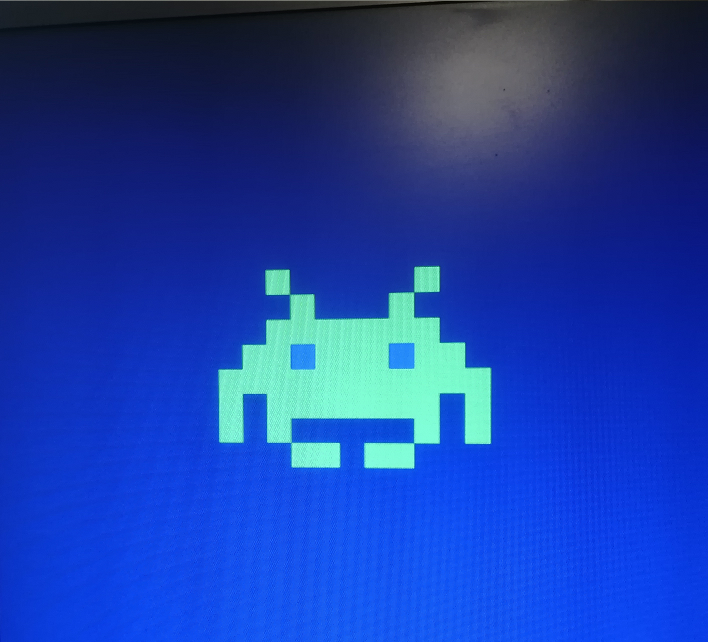
\includegraphics[scale=0.5]{img/blue.png} 
    \end{center}
\end{minipage}
\begin{center}
Arcade-SpaceInvader mit blauem Hintergrund
\end{center}





